\definecolor{TUMBlue}{HTML}{0065BD}
\definecolor{TUMSecondaryBlue}{HTML}{005293}
\definecolor{TUMSecondaryBlue2}{HTML}{003359}
\definecolor{TUMBlack}{HTML}{000000}
\definecolor{TUMWhite}{HTML}{FFFFFF}
\definecolor{TUMDarkGray}{HTML}{333333}
\definecolor{TUMGray}{HTML}{808080}
\definecolor{TUMLightGray}{HTML}{CCCCC6}
\definecolor{TUMAccentGray}{HTML}{DAD7CB}
\definecolor{TUMAccentOrange}{HTML}{E37222}
\definecolor{TUMAccentGreen}{HTML}{A2AD00}
\definecolor{TUMAccentLightBlue}{HTML}{98C6EA}
\definecolor{TUMAccentBlue}{HTML}{64A0C8}


\usepackage{pgfplots}
\usepackage{pgfplotstable}
\usepackage{tikz}
\tikzset{>=stealth}
\usetikzlibrary{patterns}
\usetikzlibrary{pgfplots.statistics}
\usetikzlibrary{positioning, shapes}
\usetikzlibrary{calc}



% node definitions
\tikzstyle{neuron} = [circle, minimum size=0.5cm, text width=0.2cm, text height=0.2cm, text centered, align=center, font=\fontsize{18}{0}\selectfont]
\tikzstyle{loss} = [very thick, rectangle, minimum width=3cm, minimum height=1.5cm, text centered, draw=black, align=center, font=\fontsize{18}{0}\selectfont]

\tikzstyle{module} = [rectangle, minimum width=2.5cm, minimum height=2cm, text centered, draw=black, rounded corners, align=center, font=\fontsize{16}{22}\selectfont]
\tikzstyle{transmodule} = [thick, rectangle, minimum width=2.5cm, minimum height=2cm, text centered, draw=black, rounded corners, align=center]
\tikzstyle{frame} = [very thick, rectangle, minimum width=2cm, minimum height=2cm, text centered, draw=black, rounded corners, align=center, font=\fontsize{16}{0}\selectfont, fill=TUMAccentBlue!10]
\tikzstyle{key} = [very thick, rectangle, minimum width=1.4cm, minimum height=1.4cm, text centered, rounded corners, align=center, font=\fontsize{16}{0}\selectfont, fill=TUMAccentGray!20]
\tikzstyle{dark_module} = [rectangle, minimum width=2.5cm, minimum height=2cm, text centered, draw=black, rounded corners, align=center, fill=TUMAccentLightBlue]

% arrow definitions

\tikzstyle{arrow} = [thick, ->,>=stealth,rounded corners=4pt, draw=black, align=center]
\tikzstyle{bluearrow} = [very thick,->,>=stealth,rounded corners=4pt, draw=TUMBlue, align=center]
\tikzstyle{darkgrayarrow} = [very thick,->,>=stealth,rounded corners=4pt, draw=TUMDarkGray, align=center]
\tikzstyle{dashedarrow} = [very thick,->,>=stealth,rounded corners=4pt, draw=black, align=center, dashed]
\tikzstyle{graydashedarrow} = [thick,->,>=stealth,rounded corners=4pt, draw=black, align=center, dashed, color=TUMGray]
\tikzstyle{orangedashedarrow} = [thick,->,>=stealth,rounded corners=4pt, draw=black, align=center, dashed, color=TUMAccentOrange]

\tikzstyle{marker} = [circle, minimum size=0.4cm, scale=0.8, text centered, draw=black, align=center, fill=orange!10, font=\large]


	\newcommand{\drawmain}{
		\centering  
		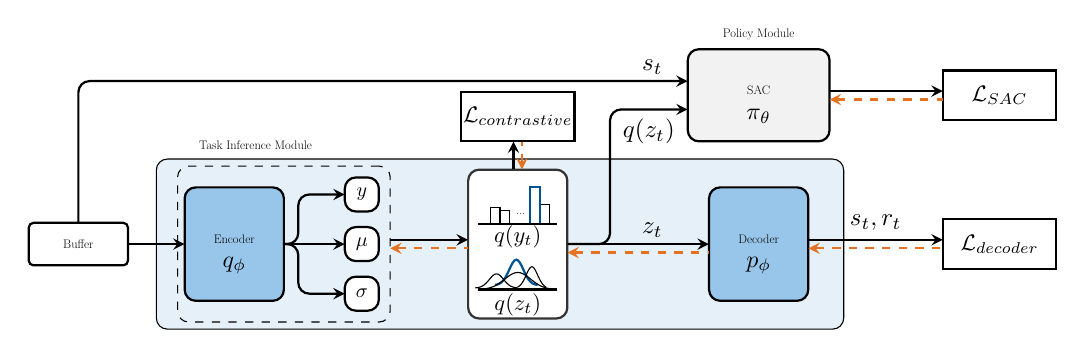
\begin{tikzpicture} [scale=0.18, transform shape]
			

			\node(all)[module, minimum width=48.5cm, minimum height=12cm, draw=black, fill=TUMBlue!10] at (-1.25,-0.5) {};
			\node(encoder)[module, dashed, minimum width=15cm, minimum height=11cm, draw=black, fill=TUMBlue!10] at (-16.5,-0.5) {};
			\path (encoder.north)+(-2,1.5) node (enc) {\fontsize{45}{0}\selectfont Task Inference Module};
			
			\node(gru)[module, thick, minimum width=7cm, minimum height=8cm, fill=TUMAccentLightBlue, font=\fontsize{45}{0}\selectfont] at (-20,-0.5) {Encoder \\[2ex]   };
			\path (-20, -2) node[scale=4.8] {$q_{\bm \phi}$};
			
			\node(buffer)[module, thick, minimum width=7cm, minimum height=3cm, rounded corners=0.6mm, font=\fontsize{45}{0}\selectfont] at (-31, -0.5) {Buffer};
			

			\node(y-pred)[module, thick, minimum width=2.4cm, minimum height=2.4cm, fill=TUMWhite] at (-11, 3) {};
			\path (-11, 3) node[scale=4] {$\bm y$};

			\node(mu-pred)[module, thick, minimum width=2.4cm, minimum height=2.4cm, fill=TUMWhite] at (-11, -0.5) {};
			\path (-11, -0.5) node[scale=4] {$\bm \mu$};
			
			\node(sigma-pred)[module, thick, minimum width=2.4cm, minimum height=2.4cm, fill=TUMWhite] at (-11, -4) {};
			\path (-11, -4) node[scale=4] {$\bm \sigma$};
			
			
			\node(gmvae)[module, thick, minimum width=7cm, minimum height=10.5cm, draw=TUMDarkGray, fill=TUMWhite] at (0,-0.5) {};
			\node(contrastive)[loss, thick, minimum width=8cm, minimum height=3.5cm, font=\fontsize{80}{80}\selectfont] at (0,8.5) {};
			\path (0, 8.5) node[scale=4.5] {$\mathcal{L}_{contrastive}$};
			
			
			\node(prob1) [loss, thin, minimum width=0.7cm, minimum height=1.2cm] at (-1.6, 1.5) {};
			\node(prob2) [loss, thin, minimum width=0.7cm, minimum height=1.0cm] at (-0.9, 1.4) {};
			\node(prob4) [loss, thin, minimum width=0.7cm, minimum height=1.4cm] at (1.9, 1.6) {};
			\node(prob3) [loss, thick, minimum width=0.7cm, minimum height=2.6cm, draw=TUMSecondaryBlue] at (1.2, 2.2) {};
			\path (0.2,1.6) node(y-dis) {\fontsize{45}{0}\selectfont ...};
			\draw[thick] (-2.8,0.9)--(2.8, 0.9);
			\path (0, 0.0) node[scale=4.5] {$q(\bm  y_{t})$};
			
			
			\def\normal-f{\x,{1.8/exp(2*(\x+0.1)^2)-3.4}}
			\draw[thick, draw=TUMSecondaryBlue, domain=-1.6:1.4] plot (\normal-f) node[right] {};
			
			\def\normal1{\x,{1/exp(2*(\x+1.5)^2)-3.6}}
			% Draw and label normal distribution function
			\draw[color=black, domain=-3:0] plot (\normal1) node[right] {};
			\def\normal2{\x,{1.2/exp(0.6*(\x)^2)-3.7}}
			% Draw and label normal distribution function
			\draw[color=black, domain=-2.2:2.2] plot (\normal2) node[right] {};
			\def\normal3{\x,{1.5/exp(3*(\x-1)^2)-3.6}}
			% Draw and label normal distribution function
			\draw[color=black, domain=0:2] plot (\normal3) node[right] {};
			
			\draw[thick] (-2.8,-3.7)--(2.8, -3.7);
			\path (0, -4.8) node[scale=4.5] {$q(\bm  z_{t})$};
			
			
			\node(sr-decoder)[module, thick, minimum width=7cm, minimum height=8cm, fill=TUMAccentLightBlue, font=\fontsize{45}{0}\selectfont] at (17,-0.5) {Decoder\\[2ex]    };
			\path (17, -2) node[scale=4.8] {$p_{\bm \phi}$};
			
			\node(loss-decoder)[loss, thick, minimum width=8cm, minimum height=3.5cm, font=\fontsize{52}{0}\selectfont] at (34,-0.5) {};
			\path (34, -0.5) node[scale=4.5] {$\mathcal{L}_{decoder}$};
			
			\path (9.5, 0.5) node[scale=5] {$\bm z_{t}$};
			

			\node(sac)[module, thick, minimum width=10cm, minimum height=6.5cm, fill=TUMGray!10, font=\fontsize{45}{0}\selectfont] at (17,10) {SAC \\[2ex]   };
			\path (17, 8.5) node[scale=4.8] {$\pi_{\bm \theta}$};
			
			\path (sac.north)+(0,1) node (po) {\fontsize{45}{0}\selectfont Policy Module};
			\node(loss-sac)[loss, thick, minimum width=8cm, minimum height=3.5cm, font=\fontsize{52}{0}\selectfont] at (34,10) {};
			\path (34, 10) node[scale=4.5] {$\mathcal{L}_{SAC}$};
			\path (9.5, 12) node[scale=5] {$\bm s_{t}$};
			
			% arrows
			\draw[arrow] (gru.east)--(mu-pred.west);
			\draw[arrow] (gru.east)--([xshift=1cm]gru.east)--([xshift=1cm]$(y-pred.west -|gru.east)$)--(y-pred.west);
			\draw[arrow] (gru.east)--([xshift=1cm]gru.east)--([xshift=1cm]$(sigma-pred.west -|gru.east)$)--(sigma-pred.west);
			
			\draw[arrow] ([yshift=0.3cm]encoder.east)--([yshift=0.3cm]gmvae.west);
			\draw[orangedashedarrow, <-] ([yshift=-0.3cm]encoder.east)--([yshift=-0.3cm]gmvae.west);
			
			\draw[arrow] ([xshift=-0.3cm]gmvae.north)--([xshift=-0.3cm]contrastive.south);
			\draw[orangedashedarrow, <-] ([xshift=0.3cm]gmvae.north)--([xshift=0.3cm]contrastive.south);
			
			\draw[arrow] (buffer.east)--(gru.west);
			\draw[arrow] (buffer.north)--([yshift=4cm]buffer.north)--([xshift=0cm, yshift=1cm]$(sac.west -|buffer.north)$)--([yshift=1cm]sac.west);
			
			\draw[arrow] (gmvae.east)--(sr-decoder.west);
			\draw[arrow] (gmvae.east)--([xshift=3cm]gmvae.east)--([xshift=3cm, yshift=-1cm]$(sac.west -|gmvae.east)$)--([yshift=-1cm]sac.west) node[midway,below, color=black, scale=5]{$q(\bm z_{t})$};
			
			\draw[orangedashedarrow, <-] ([yshift=-0.6cm]gmvae.east)--([yshift=-0.6cm]sr-decoder.west);
			
			\draw[arrow] ([yshift=0.3cm]sr-decoder.east)--([yshift=0.3cm]loss-decoder.west) node[midway,above,color=black, scale=5]{$\bm s_{t}, r_{t}$};
			\draw[orangedashedarrow, <-] ([yshift=-0.3cm]sr-decoder.east)--([yshift=-0.3cm]loss-decoder.west);
			
			\draw[arrow] ([yshift=0.3cm]sac.east)--([yshift=0.3cm]loss-sac.west);
			\draw[orangedashedarrow, <-] ([yshift=-0.3cm]sac.east)--([yshift=-0.3cm]loss-sac.west);
			
			
		\end{tikzpicture}
	}
	
	
	\newcommand{\drawcontrastive}{
	\centering
	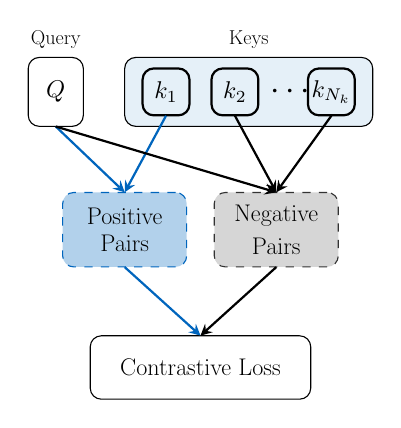
\begin{tikzpicture} [scale=0.35, transform shape]
		\node(query)[module, minimum width=2cm, minimum height=2.5cm, label={[align=center, font=\fontsize{22}{0}\selectfont]Query\\[.5ex]}] at (2,0) {};
		\path (2, 0) node[scale=2.5] {$\bm Q$};
		
		\node(keys)[module, minimum width=9cm, minimum height=2.5cm, fill=TUMBlue!10, label={[align=center, font=\fontsize{22}{0}\selectfont]Keys\\[.5ex]}] at (9,0) {};
		
		
		\node(key-1)[module, thick, minimum width=1.7cm, minimum height=1.7cm] at (6, 0) {};
		\path (6, 0) node[scale=2.5] {$\bm k_1$};
		\node(key-2)[module, thick, minimum width=1.7cm, minimum height=1.7cm] at (8.5, 0) {};
		\path (8.5, 0) node[scale=2.5] {$\bm k_2$};
		\path (10.5, 0) node[scale=3.5] {$\cdots$};   
		\node(key-n)[module, thick, minimum width=1.7cm, minimum height=1.7cm] at (12, 0) {};
		\path (12, 0) node[scale=2.5] {$\bm k_{N_k}$};   
		
		\node(pos)[module, minimum width=4.5cm, minimum height=2.7cm, draw=TUMBlue, fill=TUMBlue!30, dashed, font=\fontsize{25}{0}\selectfont] at (4.5,-5) {Positive \\[1ex] Pairs};
		\node(neg)[module, minimum width=4.5cm, minimum height=2.7cm, draw=TUMDarkGray, fill=TUMDarkGray!20, dashed, font=\fontsize{25}{0}\selectfont] at (10,-5) {Negative \\[1ex] Pairs};
		
		\node(loss)[module, minimum width=8cm, minimum height=2.3cm, font=\fontsize{25}{0}\selectfont] at (7.25,-10) {Contrastive Loss};
		
		\draw[arrow, color=TUMBlue] (query.south) -- (pos.north);
		\draw[arrow, color=TUMBlue] (key-1.south) -- (pos.north);
		
		\draw[arrow] (query.south) -- (neg.north);
		\draw[arrow] (key-2.south) -- (neg.north);
		\draw[arrow] (key-n.south) -- (neg.north);
		
		\draw[arrow, color=TUMBlue] (pos.south) -- (loss.north);
		\draw[arrow] (neg.south) -- (loss.north);
	\end{tikzpicture}
}


	\newcommand{\drawdecoder}{
	\centering
	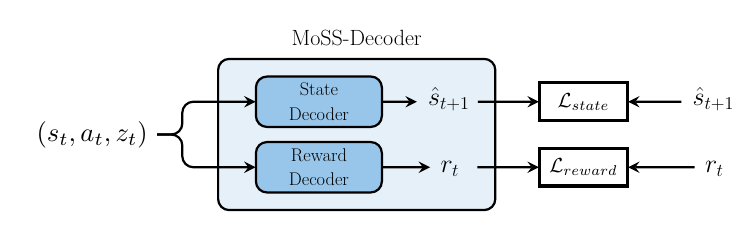
\begin{tikzpicture} [scale=0.32, transform shape]
		\node(decoder)[module, thick, minimum width=11cm, minimum height=6cm, fill=TUMBlue!10, label={[align=center, font=\fontsize{25}{0}\selectfont]MoSS-Decoder \\ [1ex]}] at (0.5,0) {};
		
		\node(state-dec)[module, thick, minimum width=5cm, minimum height=2cm, fill=TUMAccentLightBlue, font=\fontsize{22}{22}\selectfont] at (-1,1.3) {State \\[0.6ex] Decoder};
		\node(reward-dec)[module, thick, minimum width=5cm, minimum height=2cm, fill=TUMAccentLightBlue, font=\fontsize{22}{22}\selectfont] at (-1,-1.3) {Reward \\[0.6ex] Decoder};
		
		
		\path (-10, 0) node[scale=3](context) {($\bm s_{t}, \bm a_{t}, \bm z_{t}$)};
		\node(outs) [neuron, scale=1.7] at (3.5, 1.2) {$\hat{\bm s}_{t+1}$};
		\node(outr) [neuron, scale=1.7] at (4, -1.4) {$r_{t}$};
		
		\node(lossstate) [loss, minimum width=3.5cm, font=\fontsize{27}{27}\selectfont] at (9.5, 1.3) {};
		\path (9.5, 1.3) node[scale=2.3] {$\mathcal{L}_{state}$};
		\node(lossreward) [loss, minimum width=3.5cm, font=\fontsize{27}{27}\selectfont] at (9.5, -1.3) {};
		\path (9.5, -1.3) node[scale=2.3] {$\mathcal{L}_{reward}$};
	    
		
		\node(true-s) [neuron, scale=1.7] at (14, 1.2) {$\hat{\bm s}_{t+1}$};
		\node(true-r) [neuron, scale=1.7] at (14.5, -1.4) {$r_{t}$};
		
		\draw[arrow] (context.east)--([xshift=1cm]context.east)--([xshift=1cm]$(state-dec.west -| context.east)$)--(state-dec.west);
		\draw[arrow] (context.east)--([xshift=1cm]context.east)--([xshift=1cm]$(reward-dec.west -| context.east)$)--(reward-dec.west);
		\draw[arrow] (state-dec.east) -- ($(outs.west)+(0, 0.1)$);
		\draw[arrow] (reward-dec.east) -- ($(outr.west)+(0, 0.1)$);
		\draw[arrow] ($(outs.east)+(1.2, 0.1)$) -- (lossstate.west);
		\draw[arrow] ($(outr.east)+(0.7, 0.1)$) -- (lossreward.west);
		\draw[arrow] ($(true-s.west)+(0, 0.1)$) -- (lossstate.east);
		\draw[arrow] ($(true-r.west)+(0, 0.1)$) -- (lossreward.east);
\end{tikzpicture}}

	\newcommand{\drawinference}{
	\centering  
	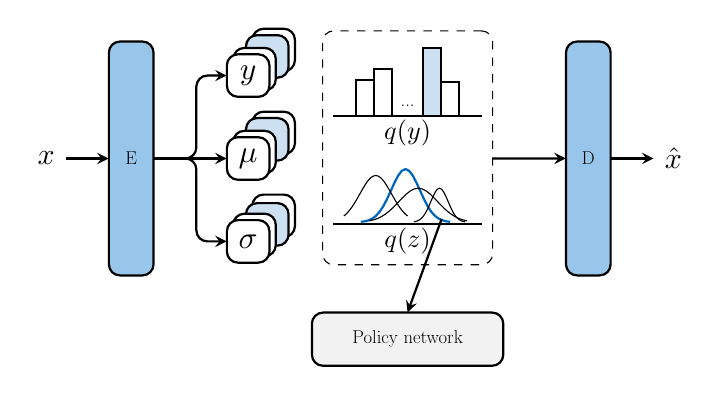
\begin{tikzpicture} [scale=0.27, transform shape]
		
		
		\node(encoder)[module, thick, minimum width=2.1cm, minimum height=11cm, fill=TUMAccentLightBlue, font=\fontsize{36}{0}\selectfont] at (-13,-1) {E};
		
		\path (-17, -1) node[scale=4] {$\bm x$};
		\draw[arrow] ($(encoder.west)+(-2,0)$) -- (encoder.west);
		
		\node(y-pred-3)[module, thick, minimum width=2cm, minimum height=2cm, fill=TUMWhite] at (-6.3, 4.1) {};
		\node(y-pred-2)[module, thick, minimum width=2cm, minimum height=2cm, fill=TUMBlue!20] at (-6.6, 3.8) {};
		\node(y-pred-1)[module, thick, minimum width=2cm, minimum height=2cm, fill=TUMWhite] at (-7.2, 3.2) {};
		\node(y-pred)[module, thick, minimum width=2cm, minimum height=2cm, fill=TUMWhite] at (-7.5, 2.9) {};
		\path (-7.5, 2.9) node[scale=4.2] {$\bm y$};
		
		\node(mu-pred-3)[module, thick, minimum width=2cm, minimum height=2cm, fill=TUMWhite] at (-6.3, 0.2) {};
		\node(mu-pred-2)[module, thick, minimum width=2cm, minimum height=2cm, fill=TUMBlue!20] at (-6.6, -0.1) {};
		\node(mu-pred-1)[module, thick, minimum width=2cm, minimum height=2cm, fill=TUMWhite] at (-7.2, -0.7) {};
		\node(mu-pred)[module, thick, minimum width=2cm, minimum height=2cm, fill=TUMWhite] at (-7.5, -1) {};
		
		\path (-7.5, -1) node[scale=4.2] {$\bm \mu$};
		
		\node(sigma-pred-3)[module, thick, minimum width=2cm, minimum height=2cm, fill=TUMWhite] at (-6.3, -3.7) {};
		\node(sigma-pred-2)[module, thick, minimum width=2cm, minimum height=2cm, fill=TUMBlue!20] at (-6.6, -4.1) {};
		\node(sigma-pred-1)[module, thick, minimum width=2cm, minimum height=2cm, fill=TUMWhite] at (-7.2, -4.6) {};
		\node(sigma-pred)[module, thick, minimum width=2cm, minimum height=2cm, fill=TUMWhite] at (-7.5, -4.9) {};
		
		\path (-7.5, -4.9) node[scale=4.2] {$\bm \sigma$};
		
		
		\node(latent)[module, minimum width=8cm, minimum height=11cm, dashed, fill=TUMWhite] at (0,-0.5) {};
		
		
		\node(prob1) [loss, thick, minimum width=0.85cm, minimum height=1.7cm] at (-2, 1.85) {};
		\node(prob2) [loss, thick, minimum width=0.85cm, minimum height=2.2cm] at (-1.15, 2.1) {};
		\node(prob3) [loss, thick, minimum width=0.85cm, minimum height=3.2cm, fill=TUMBlue!20] at (1.15, 2.6) {};
		\node(prob4) [loss, thick, minimum width=0.85cm, minimum height=1.6cm] at (2, 1.8) {};
		\draw[thick] (-3.5, 1)--(3.5, 1);
		\path (0,1.5) node(y-dis) {\fontsize{45}{0}\selectfont ...};
		\path (0, 0.2) node[scale=3.5] {$q(\bm y)$};
		
		
		\def\normal-f{\x,{2.5/exp(1.1*(\x+0.1)^2)-4}}
		\draw[thick, color=TUMBlue, draw=TUMBlue, domain=-2.2:2] plot (\normal-f) node[right] {};
		
		\def\normal1{\x,{2.2/exp(0.9*(\x+1.5)^2)-4}}
		% Draw and label normal distribution function
		\draw[color=black, domain=-3:0] plot (\normal1) node[right] {};
		\def\normal2{\x,{1.6/exp(0.6*(\x-0.5)^2)-4}}
		% Draw and label normal distribution function
		\draw[color=black, domain=-1.8:2.8] plot (\normal2) node[right] {};
		\def\normal3{\x,{1.6/exp(3*(\x-1.5)^2)-4}}
		% Draw and label normal distribution function
		\draw[color=black, domain=0.3:2.7] plot (\normal3) node[right] {};
		
		\draw[thick] (-3.5, -4.1)--(3.5, -4.1);
		\path (0, -4.9) node[scale=3.5] {$q(\bm z)$};
		
		\draw[arrow] (encoder.east)--(mu-pred.west);
		\draw[arrow] (encoder.east)--([xshift=2cm]encoder.east)--([xshift=2cm]$(y-pred.west -|encoder.east)$)--(y-pred.west);
		\draw[arrow] (encoder.east)--([xshift=2cm]encoder.east)--([xshift=2cm]$(sigma-pred.west -|encoder.east)$)--(sigma-pred.west);
		
		
		\node(decoder)[module, thick, minimum width=2.1cm, minimum height=11cm, fill=TUMAccentLightBlue, font=\fontsize{32}{0}\selectfont] at (8.5, -1) {D};
		
		\path (12.5, -1) node[scale=4] {$\hat{\bm x}$};
		
		\draw[arrow]  (decoder.east) -- ($(decoder.east)+(2,0)$);
		\draw[arrow]  ($(latent.east)+(0, -0.5)$) -- (decoder.west);
		
		\node(policy)[module, thick, minimum width=9cm, minimum height=2.5cm, fill=TUMGray!10, font=\fontsize{32}{0}\selectfont] at (0, -9.5) {Policy network};
		
		\draw[arrow]  (1.6, -3.85) -- (policy.north);
		
	\end{tikzpicture}
}